\documentclass{article}

% Language setting
% Replace `english' with e.g. `spanish' to change the document language
\usepackage[french]{babel}
\usepackage[T1]{fontenc}

% Set page size and margins
% Replace `letterpaper' with`a4paper' for UK/EU standard size
\usepackage[letterpaper,top=0.5cm,bottom=0.5cm,left=2cm,right=2cm,marginparwidth=1.75cm]{geometry}

% Useful packages
\usepackage{amsmath}
\usepackage{graphicx}
\usepackage[colorlinks=true, allcolors=blue]{hyperref}
\usepackage{wrapfig}
\usepackage{enumitem}
\usepackage{pgfplots}
\pgfplotsset{compat=1.18} 

\usepackage{tikz}
\usepackage[european, straightvoltages, RPvoltages, cute inductor]{circuitikz}  % RPvoltages definie la convention des dipoles (sens tension faux sinon)
\usetikzlibrary{babel}

% Colonnes
\newenvironment{col}[1]
{\begin{minipage}[t]{\dimexpr \textwidth * #1/100 - 0.03\textwidth}}{\end{minipage}\hspace{0.03\textwidth}}
\newenvironment{colf}[1]
{\begin{minipage}[t]{\dimexpr \textwidth * #1/100}}{\end{minipage}}
\newcommand{\twoCol}[3][50]{
    \begin{col}{#1}
        #2
    \end{col}
    \begin{colf}{\numexpr 100 - #1\relax}
        #3
    \end{colf}
}

\title{Filtres Eléctroniques Passifs}
\author{Raphaël Jamann}
\date{} % remove the date

\begin{document}
    \maketitle

    Lien playliste Youtube pour comprendre les filtres: \href{https://youtube.com/playlist?list=PLBRwdavN8jtvGuPq0_vqaGfYz1iMiCGmt&si=m3tA0icXFmadQLan}{Playliste}.
    Aide Latex circuit: \href{https://nboulaire.developpez.com/tutoriels/latex/circuitikz_base/}{lien}.

    \section{Qu'est ce qu'un filtre}
    
    Un filtre est un quadripôle linéaire (constitué de dipôles linéaires R,L et C) qui \textbf{permet
    d'atténuer certaines fréquences} en régime sinusoïdal. 

    \bigskip
    Les filtres fonctionnent grâce à l'impédance complexe des dipôles R et C qui dépendent
    de la pulsation $\omega$ et donc de la fréquence $f=\frac{\omega}{2\pi}$. \\
    En effet, l'impédance d'un condensateur est $\underline{Z}_C=\dfrac{1}{j\omega C}$ . \\
    L'impédance d'une bobine L est $\underline{Z}_L=j\omega L$


    \section{Exemples de filtres passe haut}

    \twoCol{      
        \centering

        \subsection{High Pass RC Filter}

        \vspace{2mm}
        \begin{circuitikz}        
            % Circuit code
            \draw (0,0) to[short,o-o] ++ (4,0);
            \draw (0,2) to[C, l_=C, o-] ++ (3,0) coordinate(a);
            \draw (a) to[short, -o] ++ (1,0);
            \draw (a) to[R, name=R, *-*] ++(0,-2);
            \node at (R.center) {R};  % draw label "R" at the center of the resistance

            % Voltage labels
            \draw (0,2) to[open,v=V$_{\text{in}}$\;] ++(0,-2);
            \draw (4,2) to[open,v^=\hspace{1.5mm} V$_{\text{out}}$] ++(0,-2);
        \end{circuitikz}

        Sur ce montage, lorsque la fréquence est basse, l'impédance du condensateur est très
        grande donc la tension de sortie est plus faible que celle d'entrée. \\
        Lien de la \href{https://www.falstad.com/circuit/circuitjs.html?ctz=CQAgjCAMB0l3BWcBOaAOAbAdgCwCYsBmHMBMHZNQkBSGmuhAUwFowwAoANxAzxxB4EGXvxCE0AuhAyMo8mAg4B3UQIkCsCPOMlQOAJxBadQkSd1SGHAB7HkWcXhFosaJ8hACxANQA6AM4BAPYGAC4Alky2XlpOIsJIhHie3gL+AUwAdmEGAJfRqhZmIGhwgsL6RdqWpeUaVWoVCVgiJZAqTQ0IrbUddghoSGCEnmXU5DppIABiEQA2uUyBAA4AhkHLAQAWawCuYYEASgDCMTho7mDIdGjIw8jUAmAiAIKBsgASAF6BwVmrJgHQJcYIRAyBACOey28zWgTC2QCEX+gQAJlsQuEooEmAFDgE1mEwnksnsCtAOABjJolYqVKSweCQZCstnsjmpdAYNB4Xk4Igs5yXKBMiAdYLyZLyHAsq50GDirxSwTyHSEDhAA}{simulation}.
    }{
        \centering

        \subsection{High Pass RL Filter}
        
        \vspace{2mm}
        \begin{circuitikz}        
            % Circuit code
            \draw (0,0) to[short,o-o] ++ (4,0);  % draw the bottom wire
            \draw (0,2) to[R, name=R, o-] ++ (3,0) coordinate(a);  % draw the resistance
            \node at (R.center) {R};  % draw label "R" at the center of the resistance
            \draw (a) to[short,-o] ++ (1,0);  % draw wire to the right of R
            \draw (a) to[L, l_=L, *-*] ++(0,-2);  % draw the Capacitor

            % Voltage labels
            \draw (0,2) to[open,v_=V$_{\text{in}}$\;] ++(0,-2);
            \draw (4,2) to[open,v^=\hspace{1.5mm} V$_{\text{out}}$] ++(0,-2);
        \end{circuitikz}

        Sur ce montage, lorsque la fréquence est basse, l'impédance de la bobine est faible
        donc la tension de sortie est faible également.
        $$\underline{V}_{out}(t) = \underline{Z}_L \, \underline{i}(t) = \underline{Z}_L=j\omega L \, \underline{i}(t)$$
        Lien de la \href{https://www.falstad.com/circuit/circuitjs.html?ctz=CQAgjCAMB0l3BWcAmWDLMgZgBxmcgCxg4CcS6IFkVApgLRhgBQAbiIVsiMggGwcuHMAJoQ+NJDWnQEzAE6DuvAQgDsAlVB6RmAdyobhAzt2Kj9SnvxC5C1iwdPHbOe+aiX1mm3yIPPA28XP3cRTwAPW0gkMFIBNXxwUlIOcAEAQQAdAGcJAAkAL1yAewA7XIAHWgBXABdc1hKAS3lcgEca2lyAGwBDXLraMpzm8tyAE26cnJL5Oubp2hyGnL66uoBLsprN2mhmKOIccAR7BHJTtTT-ADFmnrr5acq+memACz76w54cGiwnFsagBhBMPHsADVcsMnntfnxCEhAfY1MgBIDrvZ-NCZnMFrRmD1DD5VEYPDJIBB6DBkFg1IRkGpEmpSAREoQYp4StoTjROaQTlJYLxtFhwBAxBAsMwgA}{simulation}.    
    }


    \section{Exemples de filtres passe bas}

    \twoCol{      
        \centering

        \subsection{Low Pass RC Filter}

        \vspace{2mm}
        \begin{circuitikz}        
            % Circuit code
            \draw (0,0) to[short,o-o] ++ (4,0);  % draw the bottom wire
            \draw (0,2) to[R, name=R, o-] ++ (3,0) coordinate(a);  % draw the resistance
            \node at (R.center) {R};  % draw label "R" at the center of the resistance
            \draw (a) to[short,-o] ++ (1,0);  % draw wire to the right of R
            \draw (a) to[C, l_=C, *-*] ++(0,-2);  % draw the Capacitor

            % Voltage labels
            \draw (0,2) to[open,v_=V$_{\text{in}}$\;] ++(0,-2);
            \draw (4,2) to[open,v^=\hspace{1.5mm} V$_{\text{out}}$] ++(0,-2);
        \end{circuitikz}

        Sur ce montage, lorsque la fréquence est haute, l'impédance du condensateur est basse
        donc la tension de sortie est basse également.
        $$\underline{V}_{out}(t) = \underline{Z}_C \, \underline{i}(t) = \dfrac{1}{j\omega C} \, \underline{i}(t)$$
        Lien de la \href{https://www.falstad.com/circuit/circuitjs.html?ctz=CQAgjCAMB0l3BWK0AckDMYwE4As3sA2SQgdgCYFsQFIaa6EBTAWiwCgA3EXdckSoR58eYIXQhh49OrOgJ2AJ2H9BNUkLV1ykdgHd1Q3GJWjx7AMaGBCIQg1meyeJAjloU9IQT40hNNhYpM6uUPqmaugouDbmBrz8xkJRMUlhBvaatiCE5DFa4ZmOuakmugAeIOiQSDhCpFjgBE4mAIIAOgDOYADWABIAXl0A9gB2XQAOTACuAC5dnMMAlopdAI7TTF0ANgCGXbNMo51LY10AJludncOKs0tXTJ3znbuzswCXo9MfTNDslWMKHAPhoKGCYHsTjyIAAYkttrNFFcJrtrlcAEZogECNBVXhVUh0dC4IwCGIANS6RyRvxxhFwSBJMQoyVwwXylK6NzuD3Ywyg4EFuEg2GBSBgkEogv46DCQA}{simulation}.    
    }{
        \centering

        \subsection{Low Pass RL Filter}

        \vspace{2mm}
        \begin{circuitikz}        
            % Circuit code
            \draw (0,0) to[short,o-o] ++ (4,0);
            \draw (0,2) to[L, l_=L, o-] ++ (3,0) coordinate(a);
            \draw (a) to[short, -o] ++ (1,0);
            \draw (a) to[R, name=R, *-*] ++(0,-2);
            \node at (R.center) {R};  % draw label "R" at the center of the resistance
    
            % Voltage labels
            \draw (0,2) to[open,v=V$_{\text{in}}$\;] ++(0,-2);
            \draw (4,2) to[open,v^=\hspace{1.5mm} V$_{\text{out}}$] ++(0,-2);
        \end{circuitikz}

        Sur ce montage, lorsque la fréquence est haute, l'impédance de la bobine est
        grande donc la tension de sortie est plus faible que celle d'entrée. \\
        Lien de la \href{https://www.falstad.com/circuit/circuitjs.html?ctz=CQAgjCAMB0l3BWc0BsBmSAOMB2HAWBATk0xXIgUhCSpoFMBaMMAKADcQUAmfEbhCi68QaTH2oQw8GlDkwErAO7C+YvjgTdR4qKwA2q-oJCbtAoZKixEkMGnyYsaFNkiuJrAE6mtxoWY6EuDwrAAepkQ4otxCmDiYMUQgfCIAagA6AM5ZAPZeAC4AlvThKZoxQoJIaNzJqXyZWfQAdgVeAJelKoEWIE7UfZDKvtrq-XBBeio8qSYIOEJDI7NTC0LjwxHEyfbJi4lg+NoNIABiRfrt9NkADgCGOTdZAEaPZY6HRNSYRHxgRDQKXAQgAgtkwABrAASAC9srkWnd6ABXArZdi5IpebIARxRz3092yBVaWSKiOyABNnnlCiVsvQsuisvcCgUOi0UV1oKxcnIINR8JASLIYILgdQgUCpaJWEA}{simulation}.

    }


    \section{Exemple de filtre passe bande}
    
    {\centering
    \begin{circuitikz}        
        % Circuit code
        \draw (0,0) to[short,o-o] ++ (4.5,0);
        \draw (0,2) to[short,o-] (0.5,2) to[L, l_=L] (2,2) to[C, l_=C] (3,2) -- (3.5,2) coordinate(a);
        \draw (a) to[short, -o] ++ (1,0);
        \draw (a) to[R, name=R, *-*] ++(0,-2);
        \node at (R.center) {R};  % draw label "R" at the center of the resistance

        % Voltage labels
        \draw (0,2) to[open,v=V$_{\text{in}}$\;] ++(0,-2);
        \draw (4.5,2) to[open,v^=\hspace{1.5mm} V$_{\text{out}}$] ++(0,-2);
    \end{circuitikz}

    Lien de la \href{https://www.falstad.com/circuit/circuitjs.html?ctz=CQAgjCAMB0l3BWcA2aAOMB2ALGXyEw1sESQFJzzKEBTAWjDACgA3EZAJmxE4WQ7cQAZmJRw4eFUozoCZgHdBPUT0wJOIsZGYAnEOs18BhrT0pgdADwMBOTCM4C0mNI9sgeQgGoAdAM7+APa6AC4AlrTMNtjqjgL8SMKcHl48fv60AHahugCXUUqmxiBocLz8UIoGGmal5apVSlxelQiYAiU6zUKN7QKN1uRoSGDCHmjCDniaaSAAYuEANrm0AQAOAIaBa-4ARptZACa7AEoAMgDC0Z5obmC2lLbI07bCniggAIIByJAAEgAvAK0UIBTYBMAAayBASCWQ2tAArmD-KwguFdAEAI5I3ZLCH+ULZfzheEBE4BYJhSIgong0KhPJZJEFaDMADGygqAmQdx5Hxg8EgtlFYvFEo89CFkEwwmE2GQtmwkGw3A6bwcMogOiWHH5JWKlVkkAg0tgZWw4wIhCVz04kyqQXEYAElBVtnush1gpEvHEmmEzCAA}{simulation}.
    }



    \section{Exemple de filtre coupe bande}
    
    \twoCol{
        \centering
        \begin{circuitikz}        
            % Circuit code
            \draw (0,0) to[short,o-o] ++ (4.5,0);
            \draw (0,2) to[short, o-] ++ (1,0) to[short] ++ (0,0.75) to[C, l_=C] ++ (1.5,0) to[short] ++ (0,-0.75) -- (3.5,2) coordinate(a);
            \draw (1,2) to[short] ++ (0,-0.75) to[L, l_=L] ++ (1.5,0) to[short] ++ (0,0.75);
            \draw (a) to[short, -o] ++ (1,0);
            \draw (a) to[R, name=R, *-*] ++(0,-2);
            \node at (R.center) {R};  % draw label "R" at the center of the resistance

            % Voltage labels
            \draw (0,2) to[open,v=V$_{\text{in}}$\;] ++(0,-2);
            \draw (4.5,2) to[open,v^=\hspace{1.5mm} V$_{\text{out}}$] ++(0,-2);
        \end{circuitikz}

        Lien de la \href{https://www.falstad.com/circuit/circuitjs.html?ctz=CQAgjCAMB0l3BWEAmM0EE4DMGAcB2ZLMSANjABYxkQFJbb6EBTAWjDACgA3EU5CigSk+AkFlyD6EMHQb0F6TgHdRgiYPwIaGqJwBOILTWTCj28ZKjhInAB5GM+cchEFcLjCEFiAagB0AZ0CAe30AFwBLZntvLRcRYSQsZC8fQQDA5gA7cP0AS5jVYyE3OFK9YotdXHLdW1V+HzMEfBFTEQa1S0FWkXrYhFwkMBwQXAlwChp0kAAxSIAbPOYggGMQgFcAB1XAgCMAQ2yAEz2AJQAZAGFB5GkrXFJnMAJvcBFLw6CAMwKAR02OTWe0OmyCh0WOXCW30QTOQVkkAAEgAvILMQLhCHhcL5bKbQrQFTdDp8Cj0MldEpk-BYdpman0ip09piJkMkSslC4DxdUgUioCynsknCoWC5C8vRrckizTM5BiKSweAYdUazVarysZDQSiYCj4OmYfC81pQVUQWyLOU8jzcqV8y2Qa3QI10XCUDCyChYCgIV6dTghaxgTreSB4GyW63vehYFDWHScIA}{simulation}.
    }{
        \centering
        \begin{circuitikz}        
            % Circuit code
            \draw (0,0) to[short,o-o] ++ (4,0);  % draw the bottom wire
            \draw (0,3) to[R, name=R, o-] ++ (3,0) coordinate(a);  % draw the resistance
            \node at (R.center) {R};  % draw label "R" at the center of the resistance
            \draw (a) to[short,-o] ++ (1,0);  % draw wire to the right of R
            \draw (a) to[short, *-] ++ (0,-0.5) to[C, l_=C] ++ (0,-1) to[L, l_=L] ++ (0, -1) to[short, -*] ++ (0, -0.5);  % draw the Capacitor and inductor

            % Voltage labels
            \draw (0,3) to[open,v_=V$_{\text{in}}$\;] ++(0,-3);
            \draw (4,3) to[open,v^=\hspace{1.5mm} V$_{\text{out}}$] ++(0,-3);
        \end{circuitikz}

        On peut aussi faire un circuit comme celui-ci.\\
        Lien de la \href{https://www.falstad.com/circuit/circuitjs.html?ctz=CQAgjCAMB0l3BWcBOaAOAbAdgCwCYsBmHMBMHZNQkBSGmuhAUwFowwAoANxB0LxB4EGXv15gRdCLUZQ5MBBwBOogUJEIsI9XLyQOAdxpbxIvgJKTDqwcJCE0OW1aPnT9x+-0APQWjQoSFgI1GCUvOAiAIIAOgDOMgASAF7xAPYAdvEADkwArgAu8VxpAJZK8QCOeUzxADYAhvEFTBlxpZnxACa1cXFpSgWlvUxxRXENBQUAlxl5070AFHN1dUwAlNAcviQBpE4YEuCaEXhOAGKldQVKvQDGaXm58QBGDRk92350xNSEWD8cGZBE4AGrxVo3BZfbBOYhBBBIYgBJxnEDgvoDIZMDh3YzaOyaESEQjAmDwSAQFgIWC7QjIM7IMAkkhQWCUqAcOr4+yknmWeSwCAwMIksBYTA4HBEAFoSABfRGInOEAYNE6RX8o5qpwC-QqHUqw168BwayGnTYNR2TXG7VYCxHfRpOQK3iQcJgOjkoRyULUKR-DhAA}{simulation}.

    }    
    
    \section{Fonction de transfert : définitions}

    Fonction complexe qui indique le rapport entre la tension de sortie et celle d'entrée, notée: 
    $$\underline{H}(j\omega) = \dfrac{\underline{u}_s}{\underline{u}_e} = \dfrac{U_{s_m}}{U_{e_m}} e^{\varphi_{u_s} - \varphi_{u_e}}$$

    \begin{itemize}[label=$\ast$]
        \item Module de $H$ : gain $G(\omega) = \dfrac{U_{s_m}}{U_{e_m}}$
        \item Argument de $H$ : déphasage $\varphi(\omega) = \varphi_{u_s} - \varphi_{u_e}$
    \end{itemize}



    \section{Diagrammes de Bode}

    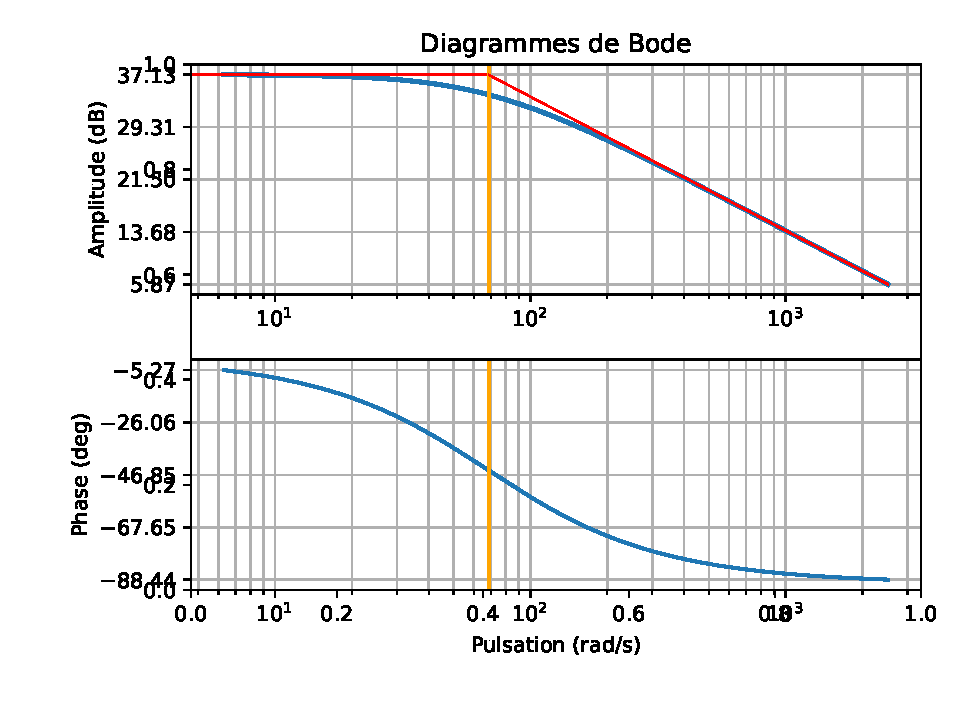
\includegraphics[width=0.9\textwidth]{fig/bode.pdf}

\end{document}